% ═════════════════════════════════════════════════════════════════════════════
\section{Parameterized Verification of Quantum Circuits}
\label{sec:quantum}
% ═════════════════════════════════════════════════════════════════════════════

The preceding sections have developed parameterized verification in the
classical setting: processes communicate through shared memory or message
passing, the parameter~$n$ counts the number of processes, and correctness
is expressed as a safety or liveness property over an infinite family of
transition systems. A structurally analogous challenge arises in quantum
computing. Most useful quantum algorithms, such as Shor's factoring
algorithm~\cite{Sho97}, Grover's search~\cite{Gro96}, and the Quantum Fourier
Transform, are \emph{parameterized by input size}: a quantum \emph{program}
takes~$n$ as input and dynamically generates the corresponding $n$-qubit
circuit. Verifying such a program requires establishing correctness for all
values of~$n$ simultaneously, a goal that parallels classical parameterized
verification but requires substantially different technical machinery.

\subsection{Quantum States and Circuits}

We recall only the notions needed in this section; a standard introduction
is~\cite{NC10}. The state of~$n$ qubits is a vector of $2^n$ complex
\emph{amplitudes}, one for each \emph{computational basis state}, that is, for
each bit string~$b$ of length~$n$. We write $\ket{b}$ for the basis state that
corresponds to~$b$, and write a state as a sum $\sum_b a_b \ket{b}$, where the
amplitudes~$a_b$ satisfy the normalization condition that the squares of their
absolute values sum to one. A \emph{gate} applies a unitary transformation to
one or a few qubits. The Hadamard gate~$H$ maps $\ket{0}$ to $(\ket{0} +
\ket{1})/\sqrt{2}$ and $\ket{1}$ to $(\ket{0} - \ket{1})/\sqrt{2}$. The
controlled-not gate CNOT acts on a control qubit and a target qubit, and
flips the target if the control is~$1$. A \emph{circuit} is a sequence of
gates, and its effect on a state is the composition of the effects of its
gates.

As a running example for this section, consider the parameterized program
that prepares the \emph{GHZ state} on $n$ qubits. Starting from the state
$\ket{0^n}$, in which all qubits are~$0$, it applies $H$ to the first qubit
and then, for each~$i$ from~$1$ to~$n-1$, a CNOT with control~$i$ and
target~$i+1$. The result is the state $(\ket{0^n} + \ket{1^n})/\sqrt{2}$, in
which all qubits are~$0$ or all are~$1$, each with probability one half.
Figure~\ref{fig:ghz} shows the circuit for $n = 3$.

\begin{figure}[t]
\centering
\begin{minipage}{0.48\linewidth}
\centering
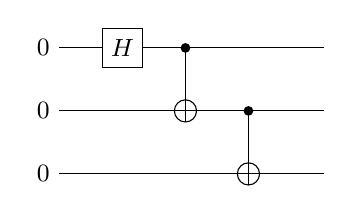
\begin{tikzpicture}[scale=0.8, every node/.style={font=\small}]
  \foreach \y/\l in {0/1, -1/2, -2/3} {
    \draw (0,\y) -- (4.2,\y);
    \node[left] at (0,\y) {$\ket{0}$};
  }
  \node[draw, fill=white, minimum size=5mm, inner sep=0pt] at (1,0) {$H$};
  % CNOT 1 -> 2
  \fill (2,0) circle (2.2pt);
  \draw (2,0) -- (2,-1.18);
  \draw (2,-1) circle (5pt);
  % CNOT 2 -> 3
  \fill (3,-1) circle (2.2pt);
  \draw (3,-1) -- (3,-2.18);
  \draw (3,-2) circle (5pt);
\end{tikzpicture}
\end{minipage}%
\hfill
\begin{minipage}{0.48\linewidth}
\centering
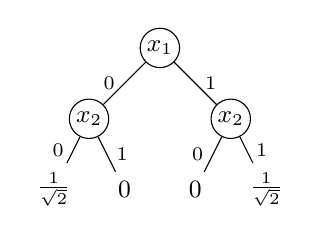
\begin{tikzpicture}[
    level distance=9mm,
    level 1/.style={sibling distance=18mm},
    level 2/.style={sibling distance=9mm},
    every node/.style={font=\small},
    inner/.style={circle, draw, inner sep=1pt, minimum size=5mm}]
  \node[inner] {$x_1$}
    child { node[inner] {$x_2$}
      child { node {$\frac{1}{\sqrt{2}}$} edge from parent node[left, font=\scriptsize] {$0$} }
      child { node {$0$} edge from parent node[right, font=\scriptsize] {$1$} }
      edge from parent node[left, font=\scriptsize] {$0$} }
    child { node[inner] {$x_2$}
      child { node {$0$} edge from parent node[left, font=\scriptsize] {$0$} }
      child { node {$\frac{1}{\sqrt{2}}$} edge from parent node[right, font=\scriptsize] {$1$} }
      edge from parent node[right, font=\scriptsize] {$1$} };
\end{tikzpicture}
\end{minipage}
\caption{Left: the circuit that prepares the GHZ state on three qubits,
consisting of a Hadamard gate followed by two CNOT gates (control marked by a
dot, target by a circle). Right: the GHZ state on two qubits represented as a
binary tree; each path from the root to a leaf selects the values of the
qubits, and the leaf stores the corresponding amplitude.}
\label{fig:ghz}
\end{figure}

\subsection{The Verification Problem}

The correctness criterion for quantum programs is characteristically different
from the safety and liveness properties of
Sections~\ref{sec:early}--\ref{sec:wmm}. Rather than asking whether a bad
state is ever reached, one asks whether the program computes the right
function: given a set of quantum state pairs $(p, q)$, does the program, for
every input size~$n$, correctly map input state~$p$ to output state~$q$? This
\emph{relational} (or \emph{functional}) specification captures input-output
correctness across all parameterized instances simultaneously. For the GHZ
program, the specification consists of the pairs $(\ket{0^n}, (\ket{0^n} +
\ket{1^n})/\sqrt{2})$, one for each~$n$. The specification also subsumes
\emph{equivalence checking} between two parameterized programs, a property of
direct practical importance for verifying that an optimized circuit
implementation is functionally identical to a reference specification,
regardless of~$n$.

Existing approaches to quantum program verification have made notable progress
but fall short of fully automatic treatment of general parameterized circuits.
Deductive approaches, based on quantum Hoare logics~\cite{Yin11} or on proof
assistants in which circuit optimizations are verified once and for
all~\cite{HRHWH21}, can handle parameterized programs but require user
guidance, while symbolic techniques such as path sums~\cite{Amy19}
automatically verify circuits of a fixed size. The Qbricks
project~\cite{Qbricks} develops a deductive framework for circuit-building
quantum programs with rich specifications; it achieves a high degree of
automation, but still requires user-provided annotations such as invariants.
Automata-based approaches~\cite{CCLLTY23,CCLLT23,LSTA25} represent sets of
quantum states by tree automata and compute the effect of each gate
automatically, which makes verification fully automatic for circuits of a
fixed size, and they have been extended to programs with control
flow~\cite{AutoQ20}. A fully automatic framework for general parameterized
quantum programs was an open problem until recently~\cite{AutoQPara}.

\subsection{Representing Infinite Families of Quantum States}

The central challenge in all parameterized verification is finding a finite
symbolic representation of an infinite family of system states, one state
space for each value of~$n$. In the classical setting, regular languages over
a finite alphabet serve this role (Section~\ref{sec:rmc}): a single finite
automaton compactly represents all reachable configurations across all
instance sizes. In the quantum setting, a parameterized program generates an
infinite family of state vectors, one for each~$n$, whose size grows
exponentially with~$n$ but which have a regular recursive structure.

The framework of~\cite{AutoQPara} achieves this through a new automata model
called \emph{synchronized weighted tree automata} (SWTAs). The starting point
is the observation that an $n$-qubit quantum state can be naturally represented
as a binary tree of depth~$n$, as in Figure~\ref{fig:ghz}: each internal node
corresponds to a qubit, and each leaf stores the complex amplitude associated
with a particular computational basis state. Standard tree automata recognize
sets of such trees, providing a symbolic representation of sets of quantum
states that is analogous to finite automata over words. SWTAs extend this with
two additional features. First, \emph{colors} attached to transitions serve as
synchronization labels: all transitions applied at the same level of a tree
must carry the same color, which enforces the level-wise uniformity that
families of quantum states require. A tree is thereby associated with a
sequence of colors, one for each level, and related input and output trees
share the same color sequence; this is the mechanism by which input-output
pairs are linked. Second, \emph{weights} on transitions encode
complex amplitudes, enabling the automaton to represent not merely which
quantum states are possible, but what amplitude each state carries. Together,
these extensions yield a model that defines a \emph{function} from color
sequences to quantum states, rather than simply a set of states. This
functional view is essential for relational verification: it allows a
specification to assert what output state is expected for each input state,
across all input sizes simultaneously.

The GHZ example illustrates the gain in succinctness. The tree for the GHZ
state on $n$ qubits has $2^n$ leaves, but its structure is simple: the left
subtree of the root contains a single nonzero amplitude at its leftmost leaf,
the right subtree contains a single nonzero amplitude at its rightmost leaf,
and all other subtrees are zero. A handful of automaton states, one for each
kind of subtree, describes this structure at every depth, and a weight
of~$1/\sqrt{2}$ at the root gives the amplitudes. The infinite family of GHZ
states, one for each~$n$, is therefore represented by a single small
automaton, in the same way as the infinite family of token-passing
configurations $\NoTok^*\Tok\NoTok^*$ is represented by a small finite
automaton in Section~\ref{sec:rmc}.

\subsection{Transducers for Quantum Gate Semantics}

In regular model checking, the transition relation of a parameterized system
is encoded as a finite-state transducer, and reachability reduces to computing
the transitive closure of that transducer (Section~\ref{sec:rmc}). The quantum
analogue replaces the transition relation with a \emph{quantum gate}, and the
transducer must encode the linear transformation that the gate applies to the
quantum state tree. The framework of~\cite{AutoQPara} introduces a class of
transducers that operate directly on SWTAs: given an input SWTA representing a
family of quantum states, applying a gate transducer produces an output SWTA
representing the family of states after the gate has been applied.

A central concern in any symbolic framework for quantum computation is
\emph{succinctness}: a quantum gate on $n$ qubits is a $2^n \times 2^n$
unitary matrix, and a naive representation is exponential in~$n$. The
transducer representation avoids this blow-up. As an illustration, the
transducer for the Quantum Fourier Transform on $n$ qubits has a number of
states that is \emph{polynomial} in~$n$, exploiting the recursive structure
of the QFT to obtain an exponentially more compact representation than a
matrix encoding would require. This mirrors the advantage of transducers
over explicit transition tables in classical regular model checking.

A further key ingredient is a \emph{composition operator} for transducers.
Given transducers for two sub-circuits, the operator automatically constructs
a transducer for their sequential composition. Starting from transducers for
individual gates, repeated composition assembles the transducer for an
entire circuit without user intervention. The operator extends to
\emph{parameterized programs}: given a transducer for a finite circuit
constituting one layer of a parameterized algorithm, composition generates
a transducer for the full parameterized version with an arbitrary number
of such layers. This step lifts finite-circuit verification to parameterized
verification, and it is the quantum analogue of computing the transitive
closure of a transducer in classical regular model checking.

\subsection{Verification Algorithms and Experimental Results}

With SWTAs as the specification formalism and transducers as the program model,
verification compares the functions from color sequences to quantum states
that SWTAs define. We write $\llbracket \mathcal{A} \rrbracket$ for the
function defined by an SWTA~$\mathcal{A}$. Let $\mathcal{A}$ be the SWTA that
specifies the expected outputs, and let $\mathcal{A}'$ be the SWTA obtained by
applying the program transducer to the input specification. Verification then
reduces to \emph{functional inclusion}, that is, to checking that
$\llbracket \mathcal{A}' \rrbracket$ is contained in $\llbracket \mathcal{A}
\rrbracket$ when both are viewed as sets of pairs of a color sequence and a
state. Equivalence checking between two parameterized programs reduces to
\emph{functional equivalence} of the output SWTAs they produce when applied to
a complete set of linearly independent inputs; correctness of this reduction
follows from the fact that quantum programs implement linear transformations,
so agreement on a complete input basis implies agreement on all inputs.
Functional inclusion and functional equivalence of SWTAs are decidable, and
the framework provides algorithms for both. In contrast, inclusion and
equivalence of the \emph{languages} of SWTAs, viewed as sets of trees, are
undecidable, which is one reason why the functional view is
essential~\cite{AutoQPara}.

The implementation, called \textsc{AutoQ-Para}~\cite{AutoQPara}, was evaluated
on a diverse set of benchmarks spanning algorithmic, arithmetic,
error-correction, and simulation circuits. It successfully verified the
Bernstein-Vazirani algorithm, a ripple-carry adder, a syndrome extraction
circuit from a quantum error-correcting code, and optimized implementations
of Grover's search and Hamiltonian simulation, comparing them against their
unoptimized reference counterparts. Verification times ranged from
14 milliseconds to 11 seconds, and to the best of our knowledge
these are the first fully automatic parameterized verifications of circuits
of this kind.

\subsection{Connections to Classical Parameterized Verification}

The structural parallels with classical parameterized verification are
instructive. In both settings the parameter~$n$ indexes an infinite family of
systems, and the goal is to verify a property of the entire family from a
finite symbolic representation. Regular languages and SWTAs both fill this
role, using words for classical configurations and trees for quantum states.
Transducers encode transition relations in the classical case and gate semantics
in the quantum case, and computing transitive closures or repeated compositions
is the operation that lifts finite reasoning to the parameterized family in
both. The functional inclusion check mirrors the final step of the classical
analyses, amounting to verifying that no reachable output state lies outside
the specification. What distinguishes the quantum setting is the
algebraic structure of the state space: quantum states carry complex amplitudes
subject to normalization and unitarity constraints, and gates are unitary linear
transformations rather than arbitrary relations. The SWTA model is designed to
respect this structure, with weights on transitions as the mechanism for
tracking amplitudes within an automata-theoretic framework. The result can be
seen as an extension of regular model checking to quantum programs, adapted to
the linear-algebraic semantics of quantum computation.
